\documentclass{standalone}
\usepackage[utf8]{inputenc}
\usepackage{tikz}
\usetikzlibrary{matrix,chains,positioning,decorations.pathreplacing,arrows}
\usepackage{amsfonts}

\begin{document}

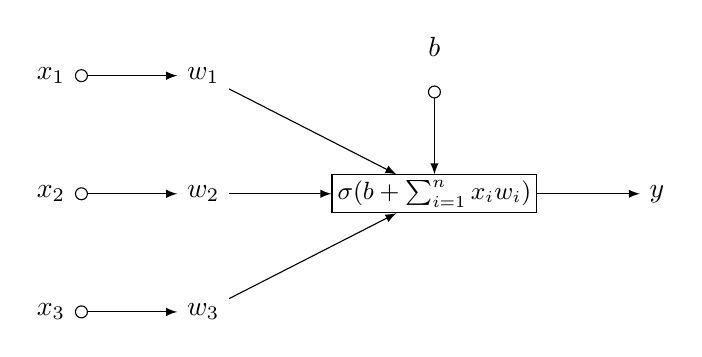
\begin{tikzpicture}[
    init/.style={draw, circle, inner sep=2pt, font=\tiny, join = by -latex},
    squa/.style={draw, inner sep=2pt, font=\small, join = by -latex},
    start chain=2,node distance=13mm
]
\node[on chain=2] (x2) {$x_2$};
\node[on chain=2,join=by o-latex] {$w_2$};
\node[on chain=2,squa] (sigma) {$\sigma(b + \sum_{i=1}^n x_i w_i)$};
\node[on chain=2,join=by -latex] {$y$};

\begin{scope}[start chain=1]
    \node[on chain=1] at (0,1.5cm) (x1) {$x_1$};
    \node[on chain=1, join=by o-latex] (w1) {$w_1$};
\end{scope}
\begin{scope}[start chain=3]
    \node[on chain=3] at (0,-1.5cm) (x3) {$x_3$};
    \node[on chain=3, join=by o-latex] (w3) {$w_3$};
\end{scope}
\node[label=above:{\centering $b$}] at (sigma|-w1) (b) {};

\draw[-latex] (w1) -- (sigma);
\draw[-latex] (w3) -- (sigma);
\draw[o-latex] (b) -- (sigma);

\end{tikzpicture}

\end{document}
